\setcounter{secnumdepth}{-1}
\section{Anhang}
\setcounter{secnumdepth}{3}

%\subsection*{Hier sind zus�tzliche Infos einzubringen}
%
%Das Beispiel f�r eine Tabbing Umgebung zeigt, dass es m�glich ist, mehrere Zeilen mit dem gleichen Einzug darzustellen:
%\begin{tabbing}
%\hspace{1.3cm}\=\hspace{2.7cm}\=\hspace{3cm}\=\kill
%$v_{Start}$ \>= 120\,km/h \>= 33,3\,m/s\\
%$v_{End}$ \>= 80\,km/h \>= 22,2\,m/s\\
%\newline
%$v_{Diff}$ \>= 40\,km/h \>= 11,1\,m/s\\
%\end{tabbing}
\subsection*{Vergleich der Sensorkonfigurationen vom \acs{FASCarE} und \acs{TIAMO}}
\begin{figure}[hbtp]%
\centering
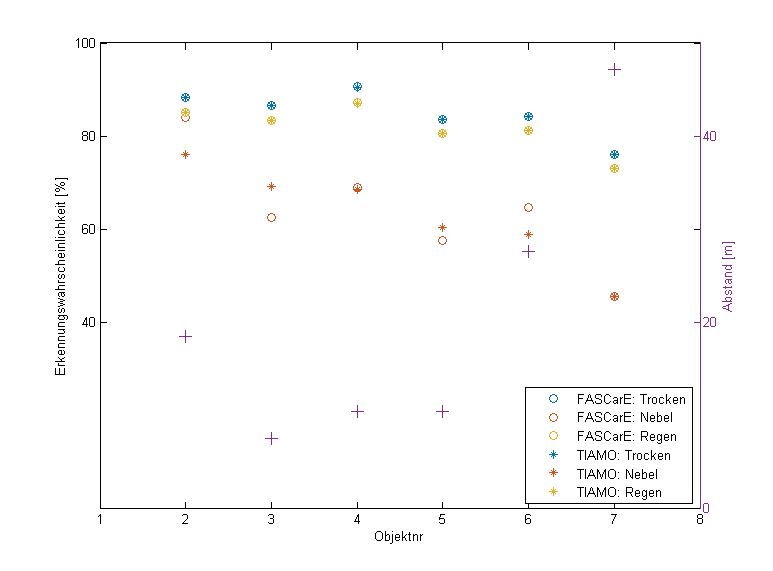
\includegraphics[width=\textwidth,trim={1cm 0.7cm 1cm 1cm},clip]{pics/VglNacht_Abstand.PNG}%
\caption[Erkennungswahrscheinlichkeiten von \acs{FASCarE} und \acs{TIAMO} bei Nacht]{Vergleich der Erkennungswahrscheinlichkeiten vom \ac{FASCarE} und \ac{TIAMO} bei Nacht zu unterschiedlichen Witterungen\label{fig:VglWahrNacht}}
\end{figure}
\newpage
\subsection*{Forschungskreuzung}
\begin{figure}[hbtp]%
\centering
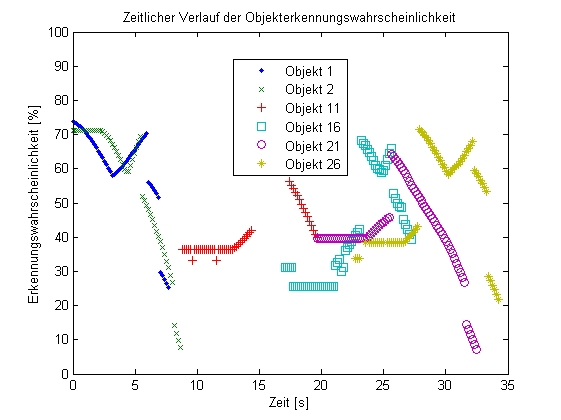
\includegraphics[width=0.9\textwidth,trim={0.7cm 0.2cm 1cm 0.7cm},clip]{pics/FoKr_WahrNebel_Obj=1,2,21,26,11,16.PNG}
\caption[Erkennungswahrscheinlichkeiten der Forschungskreuzung bei Nebel]{Erkennungswahrscheinlichkeiten der Forschungskreuzung von sechs Objekten bei Nebel\label{fig:FoKr_WahrNebel}}
\end{figure} 


\begin{landscape}
\subsection*{Sensorspezifikationen}
	
\begin{tabularx}{1.4\textwidth}{Xcccccc}%1.45 Xp{1.2cm}p{1cm}p{1.6cm}p{1.6cm}p{1cm}Xp{2cm}X
		\caption{Spezifikationen einer Auswahl von Sensoren}
	\label{tab:SensorSpec}\\\toprule
\textbf{Sensor}&$\boldsymbol{\phi_H}$/$\boldsymbol{\phi_V}$ \textbf{[�]}&$\boldsymbol{R_{min}}$/$\boldsymbol{R_{max}}$ \textbf{[m]}&$\boldsymbol{\Delta\phi_H}$\textbf{[�]}&\textbf{Tol [$\pm$m]}&$\boldsymbol{T_{Mess}}$ \textbf{[ms]}&\textbf{Hersteller}\\\midrule\endfirsthead
\caption*{Spezifikationen einer Auswahl von Sensoren}
	\label{tab:SensorSpec}\\\toprule
\textbf{Sensor}&$\boldsymbol{\phi_H}$/$\boldsymbol{\phi_V}$ \textbf{[�]}&$\boldsymbol{R_{min}}$/$\boldsymbol{R_{max}}$ \textbf{[m]}&$\boldsymbol{\Delta\phi_H}$\textbf{[�]}&\textbf{Tol [$\pm$m]}&$\boldsymbol{T_{Mess}}$ \textbf{[ms]}&\textbf{Hersteller}\\\midrule\endhead
\midrule\endfoot 
\bottomrule\endlastfoot
		
Ultraschall&120/60&0.15/1.5&10&-&1&-\\
Ultraschall&140/70&0.15/5.5&10&-&1&Bosch\\
Ultraschall&50/50&0.15/5&10&-&1&-\\\midrule
Radar&17/23.1&0.8/50&1&0.36&66&-\\
Radar&18/23.1&0.2/120&3.3&0.36&60&Continental\\
Radar&90/23.1&0.2/40&6.6&0.36&60&Continental\\
Radar&12/23.1&0.36/0.72&7&0.12&60&Bosch\\
Radar&10/23.1&0.36/0.72&7&0.12&60&Bosch\\
Radar&150/23.1&0.36/0.72&7&0.12&60&Bosch\\
Radar&20/4.5&1/60&5.3&0.5&50&Delphi\\
Radar&90/4.5&1/174&5.3&0.5&50&Delphi\\
Radar&150/10&0.5/80&5.3&0.36&50&Delphi\\
Radar&36/8&1/160&5.3&0.25&50&SmartMicro\\
Radar&70/10&1/90&5.3&0.25&50&SmartMicro\\
Radar&100/10&1/45&5.3&0.25&50&SmartMicro\\
Radar&36/12&1.5/450&5.3&0.25&79&SmartMicro\\
Radar&100/36&1.5/340&5.3&0.25&53&SmartMicro\\
Radar&100/16&1.5/330&5.3&0.25&79&SmartMicro\\
Radar&80/24&1/120&5.3&0.25&75&SmartMicro\\
Radar&80/12&1/120&5.3&0.25&75&SmartMicro\\
Radar&15/130&0.4/55&5.3&0.55&50&SmartMicro\\
Radar&66/23.1&0.82/70&5.3&0.36&60&SmartMicro\\
Radar&140/23.1&0.82/8&5.3&0.36&60&SmartMicro\\
Radar&16/23.1&0.82/120&5.3&0.36&60&SmartMicro\\
Radar&36/23.1&0.8/99&5.3&0.36&60&Jenoptik\\
Radar&165/23.1&0.75/70&5.3&1.50&50&Hella\\\midrule
Lidar&180/20.2&0.6/100&0.31&0.05&99&-\\
Lidar&27/11&1/13.5&0.31&0.1&80&Continental\\
Lidar&110/3.2&0.3/200&0.125&0.05&80&Ibeo\\
Lidar&110/3.2&0.3/120&0.125&0.05&160&Ibeo\\
Lidar&110/6.4&0.3/200&0.125&0.05&40&Ibeo\\
Lidar&145/3.2&0.3/327&0.25&0.05&25&Ibeo\\
Lidar&270/20.2&0.1/80&0.25&0.03&25&Hokuyo\\
Lidar&270/20.2&0.06/5&0.5&0.04&25&Hokuyo\\
Lidar&270/20.2&0.02/20&0.25&0.04&50&Hokuyo\\
Lidar&190/20.2&0.1/80&0.25&0.05&20&Hokuyo\\
Lidar&95/20.2&0.6/100&0.563&0.05&10&Leddartech\\
Lidar&20/3&0.6/60&2.5&0.05&333&Leddartech\\
Lidar&360/70&0.6/160&0.31&0.05&333&Ocular\\
Lidar&360/70&0.6/270&0.31&0.05&200&Ocular\\
Lidar&360/30&1/100&0.2&0.05&200&Velodyne\\
Lidar&360/40&1/100&0.2&0.05&200&Velodyne\\
Lidar&360/26.9&1/120&0.17&0.05&50&Velodyne\\
Lidar&90/20.2&1.6/250&0.023&0.05&50&Triple-IN\\
Lidar&90/20.2&0.6/170&0.023&0.05&200&Triple-IN\\
Lidar&90/20.2&2.1/300&0.023&0.05&99&Triple-IN\\
Lidar&270/20.2&0.8/160&0.045&0.05&40&Triple-IN\\
Lidar&270/20.2&2/200&0.045&0.05&66&Triple-IN\\
Lidar&360/45&0.6/1000&0.31&0.05&80&Neptec\\
Lidar&270/20.2&0.5/50&0.25&0.05&80&SICK\\
Lidar&270/20.2&0.05/8&1&0.05&80&SICK\\
Lidar&275/7.5&0.2/64&0.25&0.05&100&SICK\\
Lidar&110/3.2&0.5/300&0.125&0.05&40&SICK\\
Lidar&110/3.2&0.5/300&0.125&0.05&80&SICK\\
Lidar&120/15&0.5/75&0.13&0.05&33&SICK\\
Lidar&190/20.2&0.5/40&0.167&0.025&99&SICK\\
Lidar&190/20.2&0/80&0.25&0.025&13&SICK\\
Lidar&110/3.2&0.6/90&0.25&0.1&99&Ibeo LUX\\\midrule
Kamera (sichtbar)&50/28&1/120&0&-&33&Bosch\\
Kamera(sichtbar)&97/74&1/77.5&1&-&50&AVT\\
Kamera(\acs{FIR})&9/6.7&1/285&1&-&33&Riva\\
Kamera(\acs{FIR})&24/18&1/100&1&-&33&Riva\\
Kamera(\acs{FIR})&41.8/31.4&1/60&1&-&33&Riva\\
Kamera(\acs{FIR})&17.6/13.2&1/285&1&-&0.1&Riva\\
Kamera(\acs{FIR})&37.5/28&1/140&1&-&31&Riva\\
Kamera(\acs{FIR})&49.8/37&1/100&1&-&33&Riva\\
Kamera(\acs{NIR})&100/54&1/35&1&-&50&Riva\\
Kamera(\acs{NIR})&42.6/34.7&1/77.5&1&-&50&AVT\\
Kamera(\acs{NIR})&97/74&1/77.5&1&-&50&AVT\\\bottomrule
\end{tabularx}

\end{landscape}

